% !TeX root=main.tex
\chapter{مفاهیم پیشرفته معماری}
%\thispagestyle{empty}

\section{مقدمه}
در این فصل به تشریح مفاهیم پیشرفته‌تر معماری سیستم بلاکچین پیشنهادی می‌پردازیم. این مفاهیم شامل رمزنگاری، اجماع، اعتبارسنجی تراکنش‌ها و ارتباطات بین زنجیره‌ای است که برای تکمیل معماری پایه ضروری هستند.

\section{رمزنگاری \lr{(Cryptography)}}

\subsection{کیف پول دیجیتال \lr{(Digital Wallet)}}

هر کاربر در شبکه دارای یک کیف پول دیجیتال است که شامل:

\begin{itemize}
    \item \textbf{کلید خصوصی \lr{(Private Key)}}: عددی مخفی که فقط مالک آن را میداند
    \item \textbf{کلید عمومی \lr{(Public Key)}}: عددی که از کلید خصوصی مشتق می‌شود و برای همه قابل مشاهده است
    \item \textbf{آدرس \lr{(Address)}}: شناسه منحصربه‌فرد که از کلید عمومی محاسبه می‌شود
\end{itemize}

فرآیند تولید آدرس:

\begin{latin}
\begin{equation}
\begin{aligned}
Private\_Key &\xrightarrow{SHA256} Public\_Key \\
Public\_Key &\xrightarrow{SHA256} Address
\end{aligned}
\end{equation}
\end{latin}

\subsection{امضای دیجیتال \lr{(Digital Signature)}}

برای تأیید اصالت تراکنش‌ها، از امضای دیجیتال استفاده می‌شود:

\begin{enumerate}
    \item کاربر تراکنش را با کلید خصوصی خود امضا می‌کند
    \item امضا شامل دو جزء است: $(r, s)$
    \item کلید عمومی همراه امضا ارسال می‌شود
    \item شبکه می‌تواند با کلید عمومی، صحت امضا را تأیید کند
\end{enumerate}

\begin{latin}
\begin{equation}
Signature = Sign(Transaction\_Hash, Private\_Key)
\end{equation}
\end{latin}

\begin{latin}
\begin{equation}
Verify(Transaction\_Hash, Signature, Public\_Key) \rightarrow \{True, False\}
\end{equation}
\end{latin}

\subsection{مزایای استفاده از رمزنگاری}

\begin{itemize}
    \item \textbf{احراز هویت}: تضمین اینکه تراکنش توسط مالک واقعی انجام شده است
    \item \textbf{تمامیت داده}: اطمینان از اینکه تراکنش تغییر نکرده است
    \item \textbf{غیرقابل انکار بودن}: فرستنده نمی‌تواند تراکنش خود را انکار کند
\end{itemize}

\section{اجماع و حل تعارض \lr{(Consensus \& Fork Resolution)}}

\subsection{قوانین اجماع}

سیستم دارای قوانین اجماع زیر است:

\begin{itemize}
    \item \textbf{حداقل دشواری}: هر بلوک باید دارای دشواری حداقلی باشد
    \item \textbf{عمق نهایی‌سازی \lr{(Finality Depth)}}: پس از 6 بلوک، یک تراکنش نهایی محسوب می‌شود
    \item \textbf{زمان‌بندی}: بلوک‌ها باید ترتیب زمانی صحیحی داشته باشند
\end{itemize}

\subsection{حل تعارض در فورک \lr{(Fork Resolution)}}

هنگامی که دو زنجیره موازی در شبکه ایجاد می‌شود، از قانون زیر برای انتخاب استفاده می‌شود:

\begin{latin}
\begin{algorithm}[H]
\caption{Fork Resolution Algorithm}
\begin{algorithmic}[1]
\IF{$length(Chain_A) > length(Chain_B)$}
    \RETURN $Chain_A$
\ELSIF{$length(Chain_B) > length(Chain_A)$}
    \RETURN $Chain_B$
\ELSE
    \IF{$timestamp(Chain_A.last) < timestamp(Chain_B.last)$}
        \RETURN $Chain_A$
    \ELSE
        \RETURN $Chain_B$
    \ENDIF
\ENDIF
\end{algorithmic}
\end{algorithm}
\end{latin}

قانون اصلی: \textbf{زنجیره طولانی‌تر برنده است} \lr{(Longest Chain Rule)}.

\subsection{تحمل خطای بیزانسی \lr{(Byzantine Fault Tolerance)}}

سیستم می‌تواند تا $\frac{n-1}{3}$ نود خطاکار را تحمل کند، جایی که $n$ تعداد کل نودها است.

\begin{latin}
\begin{equation}
f = \lfloor \frac{n-1}{3} \rfloor
\end{equation}
\end{latin}

برای رسیدن به اجماع، نیاز به حداقل $\frac{2n}{3} + 1$ رأی درست داریم.

\begin{latin}
\begin{equation}
Consensus = \begin{cases} 
True & \text{if } honest\_votes \geq \lceil \frac{2n}{3} \rceil + 1 \\
False & \text{otherwise}
\end{cases}
\end{equation}
\end{latin}

\section{اعتبارسنجی تراکنش‌ها \lr{(Transaction Validation)}}

\subsection{مجموعه UTXO}

مجموعه UTXO \lr{(Unspent Transaction Output)} شامل تمام خروجی‌های خرج نشده تراکنش‌هاست:

\begin{itemize}
    \item \textbf{UTXO Set}: نگهداری خروجی‌های خرج نشده
    \item \textbf{Spent Set}: نگهداری خروجی‌های خرج شده
    \item \textbf{Balance Calculation}: محاسبه موجودی هر آدرس
\end{itemize}

\subsection{فرآیند اعتبارسنجی}

هر تراکنش باید مراحل زیر را با موفقیت پشت سر بگذارد:

\begin{enumerate}
    \item \textbf{بررسی ورودی‌ها}: آیا تمام ورودی‌ها خرج نشده هستند؟
    \item \textbf{بررسی موجودی}: آیا مجموع ورودی‌ها $\geq$ مجموع خروجی‌ها؟
    \item \textbf{بررسی امضا}: آیا امضاهای دیجیتال معتبر هستند؟
    \item \textbf{بررسی کارمزد}: آیا کارمزد کافی پرداخت شده است؟
    \item \textbf{تشخیص دوبار‌خرج}: آیا UTXO قبلاً خرج نشده است؟
\end{enumerate}

\begin{latin}
\begin{algorithm}[H]
\caption{Transaction Validation}
\begin{algorithmic}[1]
\REQUIRE Transaction $tx$
\ENSURE $Valid$ or $Invalid$
\FOR{each $input$ in $tx.inputs$}
    \IF{NOT $is\_unspent(input)$}
        \RETURN $Invalid$: Double-Spend
    \ENDIF
\ENDFOR
\STATE $input\_sum \leftarrow \sum tx.inputs.amount$
\STATE $output\_sum \leftarrow \sum tx.outputs.amount$
\IF{$input\_sum < output\_sum$}
    \RETURN $Invalid$: Insufficient Funds
\ENDIF
\STATE $fee \leftarrow input\_sum - output\_sum$
\IF{$fee < minimum\_fee$}
    \RETURN $Invalid$: Insufficient Fee
\ENDIF
\RETURN $Valid$
\end{algorithmic}
\end{algorithm}
\end{latin}

\subsection{جلوگیری از دوبار‌خرج \lr{(Double-Spend Prevention)}}

سیستم با استفاده از مکانیسم‌های زیر از دوبار‌خرج جلوگیری می‌کند:

\begin{itemize}
    \item \textbf{UTXO Tracking}: هر UTXO فقط یکبار قابل استفاده است
    \item \textbf{Spent Set}: خروجی‌های خرج شده ثبت می‌شوند
    \item \textbf{Deterministic Assignment}: هر UTXO به یک زنجیره جانبی اختصاص می‌یابد
\end{itemize}

\section{ارتباطات بین زنجیره‌ای \lr{(Cross-Chain Communication)}}

\subsection{پروتکل انتقال بین زنجیره‌ای}

برای انتقال دارایی بین زنجیره‌های جانبی، از پروتکل چهار مرحله‌ای زیر استفاده می‌شود:

\begin{enumerate}
    \item \textbf{Initiated}: شروع انتقال در زنجیره مبدأ
    \item \textbf{Locked}: قفل کردن دارایی در زنجیره مبدأ
    \item \textbf{Verified}: تأیید انتقال توسط زنجیره اصلی
    \item \textbf{Completed}: تکمیل انتقال در زنجیره مقصد
\end{enumerate}

\begin{figure}[h]
\centering
\begin{latin}
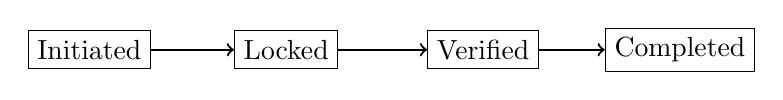
\begin{tikzpicture}[node distance=2.5cm, auto]
  \node [draw, rectangle] (init) {Initiated};
  \node [draw, rectangle, right of=init] (lock) {Locked};
  \node [draw, rectangle, right of=lock] (verify) {Verified};
  \node [draw, rectangle, right of=verify] (complete) {Completed};
  
  \draw[->, thick] (init) -- node {} (lock);
  \draw[->, thick] (lock) -- node {} (verify);
  \draw[->, thick] (verify) -- node {} (complete);
\end{tikzpicture}
\end{latin}
\caption{مراحل پروتکل انتقال بین زنجیره‌ای}
\end{figure}

\subsection{تبادل اتمی \lr{(Atomic Swap)}}

تبادل اتمی امکان مبادله دارایی بین دو زنجیره را بدون نیاز به واسطه فراهم می‌کند:

\begin{itemize}
    \item \textbf{Hash Lock}: قفل بر اساس هش یک رمز
    \item \textbf{Time Lock}: قفل زمانی برای انقضای معامله
    \item \textbf{Secret}: رمزی که برای باز کردن قفل استفاده می‌شود
\end{itemize}

\begin{latin}
\begin{equation}
Hash\_Lock = SHA256(Secret)
\end{equation}
\end{latin}

\begin{latin}
\begin{algorithm}[H]
\caption{Atomic Swap Protocol}
\begin{algorithmic}[1]
\STATE Alice creates $Hash\_Lock = SHA256(Secret)$
\STATE Alice locks funds with $Hash\_Lock$ and $Time\_Lock$
\STATE Bob locks funds with same $Hash\_Lock$ and $Time\_Lock$
\STATE Alice reveals $Secret$ to claim Bob's funds
\STATE Bob uses same $Secret$ to claim Alice's funds
\IF{$Time\_Lock$ expires}
    \STATE Both parties reclaim their original funds
\ENDIF
\end{algorithmic}
\end{algorithm}
\end{latin}

\subsection{مزایای ارتباط بین زنجیره‌ای}

\begin{itemize}
    \item \textbf{انعطاف‌پذیری}: امکان انتقال دارایی بین زنجیره‌های جانبی
    \item \textbf{بهینه‌سازی بار}: توزیع متعادل تراکنش‌ها
    \item \textbf{مقیاس‌پذیری افقی}: افزودن زنجیره‌های جانبی جدید
    \item \textbf{اتمیک بودن}: یا هر دو طرف معامله موفق هستند یا هیچکدام
\end{itemize}

\section{چالش‌ها و راه‌حل‌ها}

\subsection{چالش امنیتی زنجیره‌های جانبی}

\textbf{مشکل}: زنجیره‌های جانبی دارای دشواری کمتری هستند، ممکن است آسیب‌پذیرتر باشند.

\textbf{راه‌حل}:
\begin{itemize}
    \item زنجیره اصلی به عنوان لنگر امنیتی عمل می‌کند
    \item تأیید نهایی توسط زنجیره اصلی انجام می‌شود
    \item مکانیسم Checkpoint برای جلوگیری از حملات 51\%
\end{itemize}

\subsection{چالش همگام‌سازی}

\textbf{مشکل}: نیاز به همگام‌سازی بین زنجیره اصلی و زنجیره‌های جانبی.

\textbf{راه‌حل}:
\begin{itemize}
    \item ارجاعات منظم به زنجیره اصلی
    \item پروتکل همگام‌سازی خودکار
    \item مکانیسم بازیابی در صورت عدم همگامی
\end{itemize}

\subsection{چالش تقسیم شبکه \lr{(Network Partition)}}

\textbf{مشکل}: ممکن است بخشی از شبکه از بقیه جدا شود.

\textbf{راه‌حل}:
\begin{itemize}
    \item پروتکل اجماع مقاوم در برابر تقسیم
    \item زنجیره اصلی به عنوان منبع حقیقت
    \item مکانیسم ترمیم پس از اتصال مجدد
\end{itemize}

\section{خلاصه فصل}

در این فصل به تشریح چهار مفهوم کلیدی که پایه‌های اصلی سیستم را تشکیل می‌دهند و برای عملکرد صحیح معماری ضروری هستند پرداختیم. ابتدا \textbf{رمزنگاری} معرفی شد که شامل کیف پول‌های دیجیتال و امضای دیجیتال برای احراز هویت و تضمین تمامیت تراکنش‌ها است. سپس \textbf{اجماع} و جنبه‌های مختلف آن، از جمله قوانین اجماع، نحوه حل فورک و تحمل خطای بیزانسی مورد بررسی قرار گرفت. در ادامه، فرآیند \textbf{اعتبارسنجی} با تمرکز بر مجموعه \lr{UTXO}، اعتبارسنجی تراکنش‌ها و جلوگیری از دوبار‌خرج تشریح شد. در نهایت، \textbf{ارتباط بین زنجیره‌ای} شامل پروتکل انتقال و تبادل اتمی توضیح داده شد که نقش مهمی در هماهنگی و تعامل میان زنجیره‌های مختلف ایفا می‌کند.

